\documentclass{hw}

\usepackage{listings}

\title{Assignment 6}
\author{MATH 168, Spring 2022}
\date{Due Monday, May 23rd}

\begin{document}

\section*{Readings}

\begin{itemize}
    \item \href{http://www.philchodrow.com/intro-networks/chapters/agent_based_modeling.html}{Lecture notes} on agent-based modeling.
    \item Newman 16.1, 16.2. 
    \item \href{https://www.pnas.org/doi/full/10.1073/pnas.2025764118}{Stewardship of global collective behavior} by Bak-Coleman et al. 
\end{itemize}


\problem{(2 points)}


Make a meme related to MATH 168, post it on Campuswire with category ``meme,'' and submit a screencap of your post with this assignment. 
Sites \href{https://imgflip.com/memegenerator}{like this} one make the process of creating memes easy, but you're welcome to make your meme in any way you choose. 

You get: 
\begin{itemize}
    \item \textbf{1 point} for communicating an idea or concept related to the course content, a topic in Newman, or another concept in network science. 
    Obviously you can't be 100\% scientifically accurate in a meme, but please make sure that you're not misleading either. 
    \item \textbf{1 point} for making us giggle. 
\end{itemize}
You can earn either or both of these points. 
For example, a meme that makes fun of Prof. Chodrow is very likely to get the point for making him giggle, but may be less likely to get the point for concepts related to networks and network science. 
You're welcome to post up to two memes. 
If either of them correctly communicate a networks idea, you'll get the first point, and if either of them make us giggle, you'll get the second point. 

You can make your meme about any topic related to network science, including topics that we haven't covered in class. 
A particularly meme-able debate in the network science community concerns whether real-world networks have degree distributions which obey power laws. 
Newman discusses this topic in 10.4, and describes some related models in 13.1-13.3. 
You can find an overview of the recent debate in \href{https://www.nature.com/articles/s41467-019-09038-8}{this perspective piece} by Petter Holme. 

\problem{(2 points)}

\begin{note}
    I know that many students get excited by the idea of thinking about models of phenomena related to current events. 
    However, it's also possible to feel exhausted or drained by these events, and it's totally valid to not want to do homework problems related to them. 
    If you're feeling like you just can't with homework problems on epidemic models, let me know and we can work out different ways for you to demonstrate your learning. 
\end{note}

As mentioned in the previous problem, it's long been a topic of contention about whether real-world networks have degree distributions that obey power laws. 
One of the important properties of networks with (approximate) power law degree distributions is that the second moment $\langle k^2 \rangle = \frac{1}{n}\sum_{i \in N}k_i^2$ of the degree sequence can be quite large. 
As you may remember from our discussion of configuration model random graphs, this can have an impact on important large-scale properties of the network. 
One famous finding is that \emph{high second moments allow disease to spread more quickly}. 
In this problem, you'll use agent-based modeling to show an example of this. 

In this problem, we'll use the agent-based model described in \href{http://www.philchodrow.com/intro-networks/chapters/multi_agent_models.html#epidemic-modeling}{this section of the lecture notes}. 
To get started, copy and paste the code for importing the required packages, the \texttt{CompartmentalModel} class, the \texttt{CompartmentalAgent} class, and the \texttt{F\_SIS} function into a Jupyter Notebook.  
You won't need any of the code under ``Incorporating Global Policy.''

\part 

The Albert-Barabasi model is a random graph model that generates graphs with approximate power-law degree sequences. 
Create a \texttt{nx.barabasi\_albert\_graph} with 1,000 nodes and \texttt{m = 5}. 
This generates a graph with expected mean degree $\langle k \rangle \approx 10$. 
Compute the actual mean degree $\langle k \rangle$ and the second moment of the degree distribution $\langle k^2 \rangle$. 

\part 
Create an Erd\H{o}s-R\'enyi random graph with the same expected mean degree. 
Again compute the realized mean degree $\langle k \rangle$ and the second moment of the degree distribution $\langle k^2 \rangle$. 
Comment on the second moment when compared to the second moment of the Albert-Barabasi graph. 

\part 
On each of the two graphs you generated, create a \texttt{CompartmentalModel} with the following parameters: 

\begin{verbatim}
    model = CompartmentalModel(G, 
                               CompartmentalAgent, 
                               p_infected = 0.001,  
                               F = F_SIS, 
                               beta = 0.01, 
                               beta_background = 0.0001, 
                               gamma = 0.1)
\end{verbatim}
Then, run the model for at least 1,000 timesteps (more is better). 
Plot the proportion of infected individuals over time for each of the two graphs, and comment on your findings.  
Which kind of graph leads to greater overall levels of infection? 

\part 

For the Albert-Barabasi graph only, create a scatterplot in which there is a point for each node, and:
\begin{itemize}
    \item The horizontal axis gives the degree of the node. 
    \item The vertical axis gives the overall percentage of the time that the node was infected in the simulation. 
\end{itemize}
\begin{hint}
    You can compute the information you need for the vertical axis with the following code: 
    \begin{verbatim}
        report = model.collector.get_agent_vars_dataframe().reset_index()
        report["is_I"] = report["State"] == "I"
        report.groupby("AgentID")["is_I"].mean()
    \end{verbatim}
\end{hint}

\part 

Briefly discuss your overall findings. 
In your discussion, please use the phrase ``super-spreader'' and describe how it relates to what you've learned from your simulations. 

\problem{(2 points)}

\begin{note}
    I know that many students get excited by the idea of thinking about models of phenomena related to current events. 
    However, it's also possible to feel exhausted or drained by these events, and it's totally valid to not want to do homework problems related to them. 
    If you're feeling like you just can't with homework problems on epidemic models, let me know and we can work out different ways for you to demonstrate your learning. 
\end{note}

In 16.1.2, Newman describes the SIR (Susceptible-Infected-Recovered) model of epidemics. 
He focuses on the SIR model with differential equations, but we are instead going to study it with an agent-based model on a network. 

\part

Write a function, similar to \texttt{F\_SIS}, called \texttt{F\_SIR}. 
You only need to modify a few lines. 
Whereas in \texttt{F\_SIS} when a node ``recovers'' it is again Susceptible to infection, in \texttt{F\_SIR} the node should instead enter the state ``Recovered'' (R), from which infection is no longer possible. 
The same parameter $\gamma$ can be used: in each time step, an Infected node has probability $\gamma$ to become Recovered. 

Please show your function and place a comment beside any lines you have modified. 
No output is necessary in this part. 

\part 

Now, run your model with the following parameters: 
\begin{verbatim}
    n = 1000
    m = 5
    G = nx.barabasi_albert_graph(n, m, seed=None, initial_graph=None)
    model = CompartmentalModel(G, 
                               CompartmentalAgent, 
                               p_infected = 0.001,  
                               F = F_SIR, 
                               beta = 0.05, 
                               beta_background = 0.005, 
                               gamma = 0.1)

    for i in range(1000):
        model.step()
\end{verbatim}
Then, plot the number of nodes in each of the three states (S, I, and R) over time. 
My plot with these parameters looked like this: 

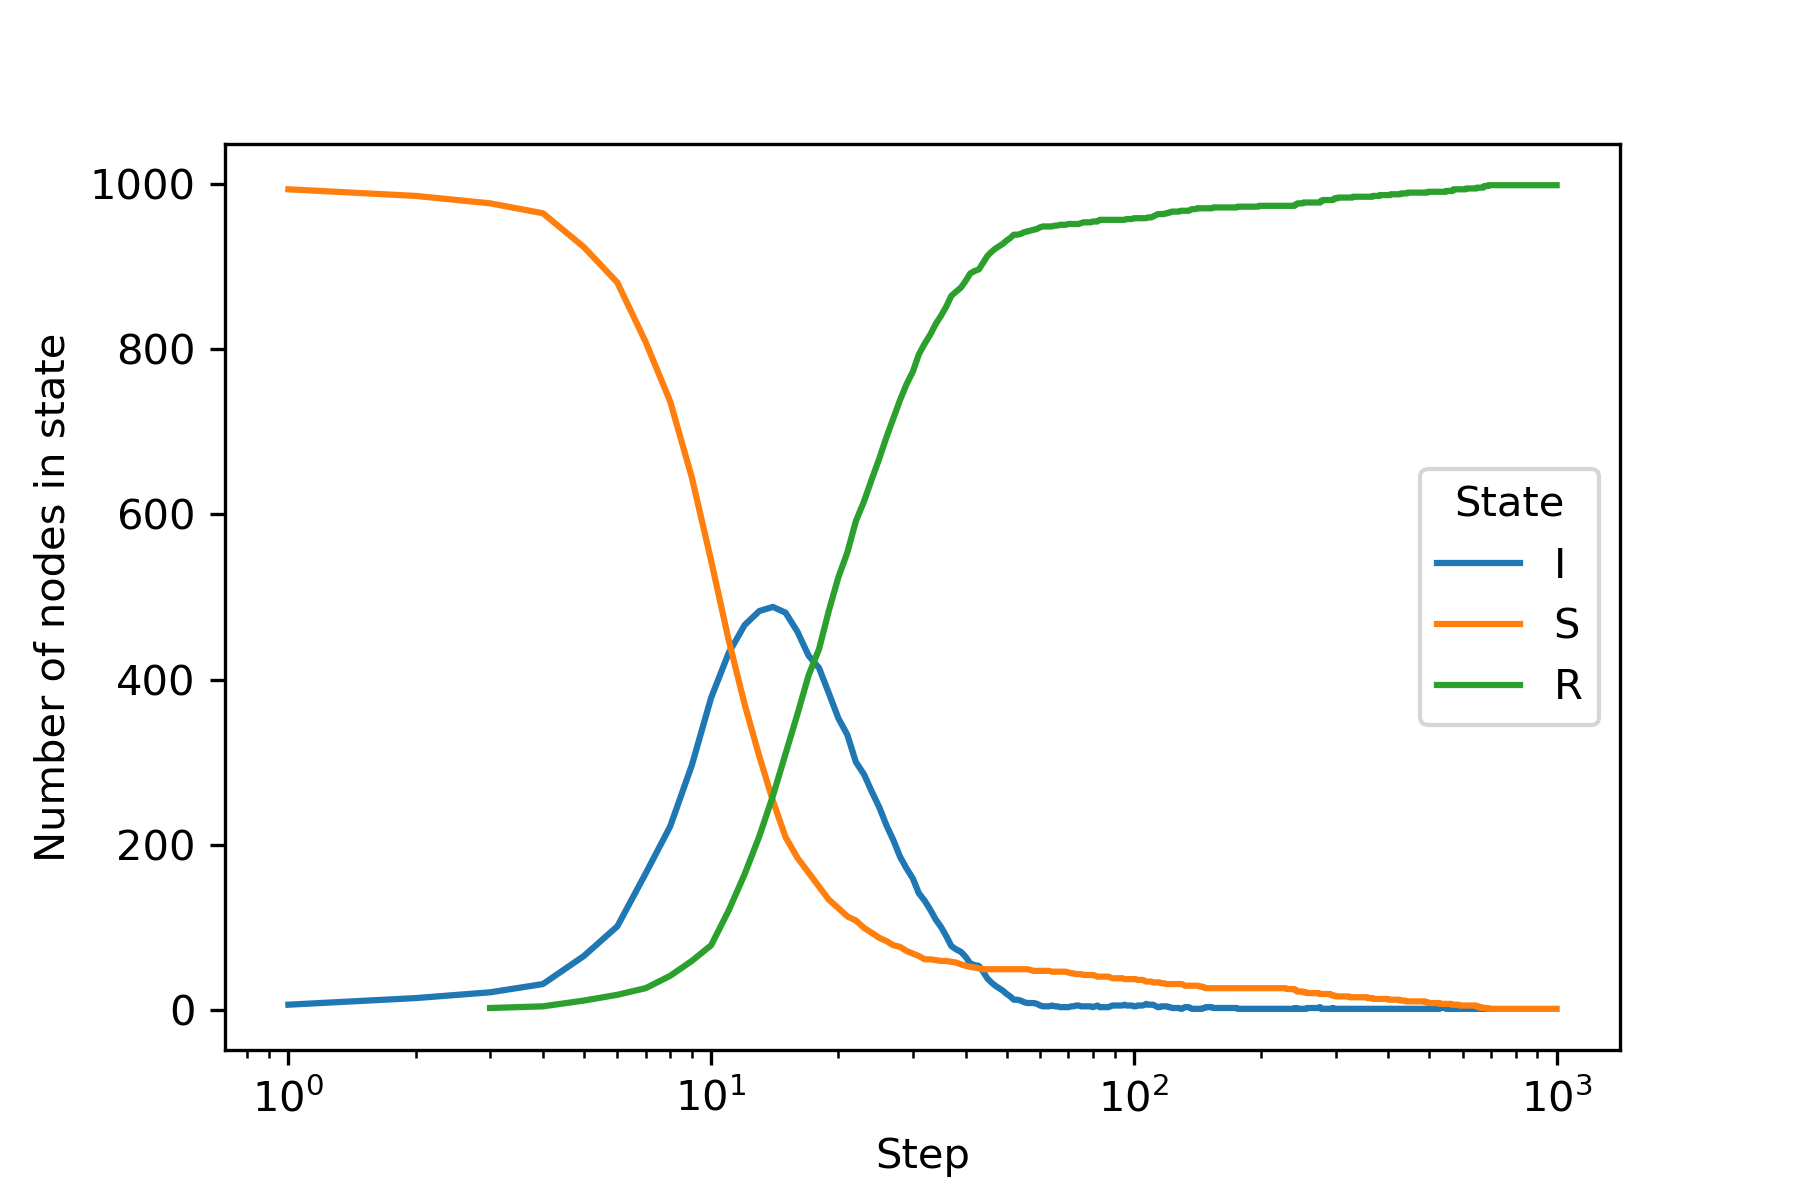
\includegraphics[width=0.7\textwidth]{SIR-example.png}

\part

Compute: 
\begin{itemize}
    \item The total number of nodes that were ever infected during your simulation. 
    \item The largest number of nodes that were ever \emph{simultaneously} infected during your simulation.  
\end{itemize}
For example, in the simulation above, 999/1000 nodes were infected by the final timestep, and there were up to 488 nodes infected during a single timestep. 
Show both your code and your result. 
Your results should be relatively pretty similar to mine, though small differences are expected. 

\part 

Run the same code as in Part (b), but change the value of \texttt{beta} to 0.01. 
Produce the same plot as in Part (b), and also compute the number of nodes infected and the number of nodes simultaneously infected as you did in Part (c). 

\part 

Briefly discuss your results. 
How did your two simulations compare in terms of total number of people infected? 
What about the largest number of people simultaneously infected? 
Comment on your overall results, using the phrase ``flatten the curve'' and describing how it applies. 



\problem{(2 points)}

Read the paper \href{https://www.pnas.org/doi/full/10.1073/pnas.2025764118}{Stewardship of global collective behavior} by Bak-Coleman et al. 
Then, write a \textbf{short} essay that addresses the following questions. 
Please spend one paragraph on each of the following items, for a total of three paragraphs. 

\begin{enumerate}
    \item What is collective behavior? According to the authors, what important features of collective behavior have \emph{changed} in the last several decades? Why is it more urgent than ever to study collective behavior? 
    \item The authors emphasize the ways in which the human social network has changed recently, and note that many models of human behavior depend strongly on network structure (p. 4 of the PDF version).  
    Their implication is that changes in network structure can lead to very different long-term or macroscopic outcomes. 
    Relate this idea to one example that we've seen in class (or homework, lecture notes, Newman, etc). 
    Then, skim one of the papers that the authors cite in this section. 
    In just a sentence or two, state what that paper concludes about the relationship of network structure and long-term or macroscopic outcomes in the system it studies. 
    \item The authors argue for a \href{https://en.wikipedia.org/wiki/Hippocratic_Oath#Modern_versions_and_relevance}{Hippocratic oath} to be taken by anyone who is studying or intervening in collective behavior. 
    Imitating the modern Hippocratic oath, suggest three sentences that should be included in a Hippocratic oath for stewardship of collective behavior. 
    How did you choose these sentences? 
    Please justify their importance by referring to specific parts of the paper. 
\end{enumerate}











\end{document}